\section{Konseptet}\label{sec:konsept}

Målet med dette avsnittet er å gi et innblikk i det utviklede konseptet,
hvilke spillaspekter som er tatt med og spilldynamikken.

\subsection{Garbage Alert}

			\begin{figure} [here]
				\begin{center}
					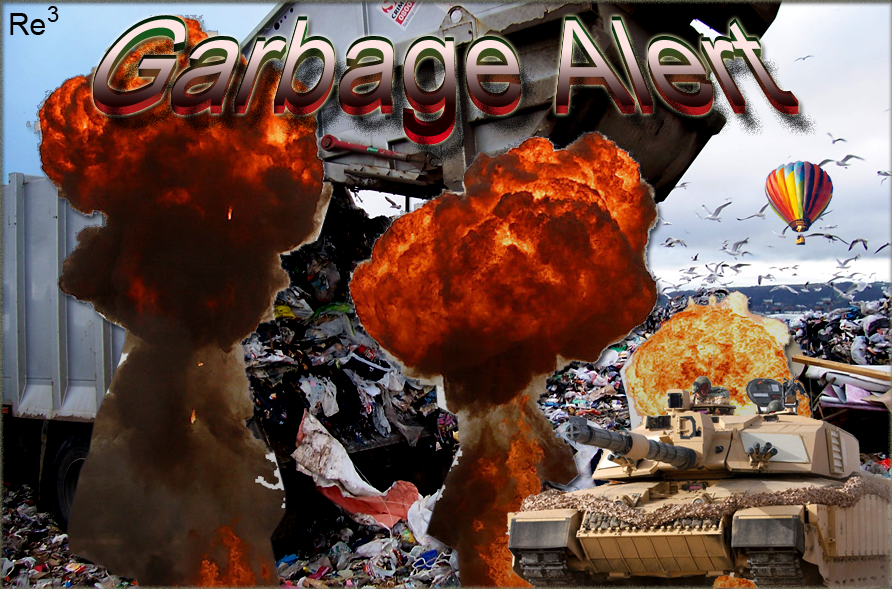
\includegraphics[scale=0.5]{images/splashscreen}
				\end{center}
			\caption{Garbage Alert}
		\end{figure}

\subsection{Introduksjon}


Garbage Alert er et sanntids strategispill for mobile enheter. Hver
spiller blir tildelt en øy dekket med søppel. En øy består av en
gjenvinningsstasjon, en våpenstasjon og en forsvarssone.
Gjenvinningsstasjonen har som oppgave å transformere øyas søppel om til
ressurser. Disse ressuresene kan brukes til å kjøpe våpen,
forsvarsmurer, utvinne nye ressurser og oppgradere
gjennvinningsstasjonen. Mulige oppgraderinger for gjenvinningsstasjonen
er raskere gjennvinning og større kapasitet for inntak av søppel. Våpen
brukes til å skyte søppel på motstandernes øyer, og forsvarsmuren har
som oppgave å blokkere slike angrep. 

Det er flere muligheter for å vinne i dette spillet. Det første
vinnsenarioet er å bli den første til å kvitte seg med alt søppelet på
øyen sin. Den andre måten å vinne på er å skyte i stykker motstandernes
gjenvinningsstasjon. Hvis en øy mister gjenvinningsstasjonen sin, vil
den bli oversvømt med søppel og synke ned i havet. Dermed kan spilleren
velge om han/hun vil fokusere på å forbedre sin egen øy eller ødelegge
for andre. 

\subsection{Spillanalyse}

Spillbeskrivelse: Spillets sjanger er valgt til flerspiller sanntidsstrategi, men det vil også være mulighet for å spille alene mot computer. (Usikker på om vi ble enig om at dette skulle være mulig?) Viktige spillelementer vil være samling, ressursforvaltning, valg av våpen og forsvar, samt timing av våpenbruk. Spillinnholdet vil hovedsaklig være Pure Play (Usikker på dette innebærer det jeg tror), der målet er å få spilleren til å ha det gøy, men det vil også være elementer av realisme da det spilleren foretar seg vil virke inn på både lokalt og globalt miljø. Det vil være en lineær spillsekvens (Er usikker på denne fordi jeg ikke finner noen  spillsekvenstype som passer??) der spilleren får tilgang til nye våpentyper og forsvarsmuligheter etterhvert som krav for hver enkelt oppgradering er nådd. For at spillet skal få et lekent og fristende utseende har vi valgt en type tegneseriestil som vil gjøre nettopp dette. (Husker ikke om vi har vi diskutert dette, og hva vi kom fram til?)\\ 
\\
Game Reference / Spillreferanse: Sjønner ikke helt hva som skal være med her, spillstrategi, spillinnlevelse, referanser\\
\\
Spillteknisk: Den tekniske formen (technical form) på spillet er flat 2D grafikk (Eller er jeg helt på bærtur??) der visningen for spilleren vil være i et ovenfra-ned perspektiv (top-down perspective). Programvareplattform er Java (Eller ikke?) og spillet er hovedsaklig tenkt for mobilenheter.

\subsection{Spillatmosfære}

This is where it is best to have a mood board or a clear description of the game’s style. 

This is a good place to start interacting with a graphic designer.\\

Atmosphere Mood Board\\
Character  Units Sketch and Description\\
A Level(Locations) Sketch and Description\\
Audio Description

\subsection{Game Play}

Using this outline to create a descriptive paragraph about how the game is played. 

The idea is that you want the person imagine they are actually playing the game.

Do not use Generic names when writing about the game play. 

Example: No one wants to here that enemy 1 will have more hit points than enemy 2. Instead we should talk about how the Lazarus Fighter has more armour than Apollo Fighter.

This outline will vary according to the type of game. \\
Opening the game application\\
Game Options \\
Story Synopsis\\
Modes\\
Game Elements\\
Game Levels\\
Player’s Controls\\
Winning\\
Losing\\
End\\
Why is all this fun?\\
\\
Game Elements / Spillelementer: 
Spilleren kan utvinne ressurser ved å "dra" søppelenheter fra forskjellige plasser på øya inn til gjennvinningsstasjonen. Hvilke ressurser, og mengden av hver ressurs, som spilleren får ut fra en enkelt søppelenhet er avhengig av nivået på gjennvinningsstasjonen og hvilke typer oppgraderinger som er gjort. Spilleren kan også bruke sine våpen til å bli kvitt søppelenheter. Her vil ubehandlede søppelenheter kunne skytes på motstandere. Effekten av angrepet avhenger av spillerens våpen, oppgraderingsnivå på våpenet og motstanderens forsvar. For å beskytte seg mot angrep kan spilleren bygge mur rundt sin øy. Hvilke våpen og forsvarsmurer som spilleren kan bygge er avhengig av hvilke ressurser gjenvinningsstasjonen er i stand til å utvinne. Dette betyr at valg av typer oppgradering for gjenvinningsstasjonen vil være avgjørende for utviklingen av spillet.\\
\\
Game Levels / Spilloppgraderinger: 
Spilleren har mulighet til å oppgradere både gjenvinningsstasjonen, våpen og forsvar. Hver type våpen og forsvar har tre nivå, der øking i nivå vil gi hhv. kraftigere angrep og sterkere forsvar. De tre våpenplassene på øya kan ha inneholde ulike våpen som kan oppgraderes hver for seg. (Skal vi ha med oppladningstid for våpen her??)\\
Eksempel på forsvarsoppgradering:\\
Tremur (nivå 1) (pil) Tremur (nivå 2) (pil) Tremur (nivå 3)\\
\\
Gjenvinngsstasjonen kan oppgraderes på følgende områder:\\
\begin{itemize}
	\item Effektivitet: Hvor fort den prosesseserer en enhet søppel (dette starter seint og går raskere for hver oppgradering).
	\item Volum/Utvinningsgrad: Hvor mye av søppelet som faktisk blir gjennvunnet. “Restavfallet” vil på magisk vis bli borte.
	\item Buffer: Stasjonen kan få en buffer hvor spilleren kan samle opp søppel, som automatiserer gjenvinningsprosessen til en viss grad.
	\item Ressurser: For å kunne utvinne nye typer ressurser må spilleren oppgraderegjenvinningsstasjonen. Denne oppgraderingen kan gjøres på flere forskjellige måter (her burde vi sette inn bilde av ressursoppgraderingsmønster)
\end{itemize}

Winning / Vinn-scenarioer:
En spiller vinner hvis
\begin{itemize}
	\item han klarer å fjerne alt søppel fra sin øy før motstanderne
	\item øyene til alle motstandere er sunket i havet fordi de blir overfylt med søppel, dvs. at han er eneste øy igjen
\end{itemize}

Losing / Tap-scenarioer:
En spiller taper hvis
\begin{itemize}
	\item gjenvinningsstasjonen på øya blir ødelagt av motstanderne slik at øya blir overfylt med søppel og synker ned i havet
	\item en av motstanderne klarer å fjerne alt søppel fra sin øy før spilleren
\end{itemize}

\subsection{Nøkkelfunksjoner}

Key features are a list of game elements that are attractive to the player.

It is a good idea to talk about the key features with someone from marketing.\\
Number of Levels\\
Number of Enemies or Characters (Example: 12 characters or amount of enemies, end bosses)\\
Time of Game Play (Example: 2 hours of fun)\\
Replay ability \\
Audio Specifications\\
Graphic Specifications\\
Device Compatibility\\
Number of Players\\
Online Activities (high scores, etc.)\\
Number/Type Modes

\subsection{Selling Features}

Denne delen trenger vi vell ikke å ha med?


